\documentclass[hidelinks, a4paper,12pt]{article}
\usepackage{ amsmath, amssymb}
\usepackage{graphicx}
\usepackage{color,amsmath,graphics,graphicx}
\usepackage{amsfonts} % replace subfigure with subcaption instead 
\usepackage{mathrsfs,hyperref}
\usepackage{latexsym,amsmath,enumerate,amsbsy,amsthm,verbatim,enumitem}
\usepackage{amstext,amsopn}
\usepackage{makeidx} 
\textwidth = 415pt

%==============================================
\usepackage{fontspec}
\usepackage{xunicode}
\usepackage{xltxtra}
\defaultfontfeatures{Scale=1.23}
\XeTeXlinebreaklocale “th_TH” % สำหรับตัดคำ
\setmainfont[Scale=1.23]{THSarabunNew}
%==============================================
%%%%%%%%%%%%%%% THEOREM Environments %%%%%%%%%% 
\newtheorem{theorem}{ทฤษฎีบท}[section]						%
\newtheorem{lemma}[theorem]{บทตั้ง}						%
\newtheorem{conjecture}[theorem]{บทคาดการณ์}				%
\newtheorem{definition}[theorem]{บทนิยาม}					%
\newtheorem{remark}[theorem]{หมายเหตุ}						%
\newtheorem{proposition}[theorem]{ประพจน์}					%
\newtheorem{corollary}[theorem]{บทแทรก}					%
\numberwithin{equation}{section}							%
\newtheorem{example}[theorem]{ตัวอย่าง}						%
%\newtheorem{exercise}{แบบฝึกหัด}[chapter]	
%\renewcommand{\chaptername}{บทที่}
\renewcommand\tablename{ตารางที่}
\renewcommand\figurename{รูปที่}
\renewcommand{\contentsname}{สารบัญ}						%
%\renewcommand{\bibname}{บรรณานุกรม}						% 
\renewcommand{\indexname}{ดรรชนี}					%
\counterwithin{figure}{section}
\numberwithin{equation}{section}		
%%%%%%%%%%%%%%%%%%%%%%%%%%%%%%%%%%%%%%%%%%%%%%%
% addition mod
\usepackage{subcaption,float,framed,algorithm2e,hyperref}
% =============

\begin{document}
	{\begin{center}
			\textbf{Report Progress}\\
			\vspace{0.5cm}
			\textbf{Division of Applied Mathematics, Department of Mathematics}\\
			\vspace{0.5cm}
			\textbf{Faculty of Science, Silpakorn University}
		\end{center}}
		{
			\vspace{0.5cm}
			\flushleft{Date : { 23 พฤศจิกายน 2561 } \hfill{ }}
			\flushleft{Advisor : { ผู้ช่วยศาสตราจารย์ ดร.นพดล  ชุมชอบ}}\\
			\flushleft{Student : {นายภัคพล พงษ์ทวี รหัส  07580028}
			\vspace{1cm}
		}
		
		
		% Here the project title
		{\textbf{\begin{flushleft}Project Title : ขั้นตอนวิธีเชิงตัวเลขชนิดใหม่สำหรับการต่อเติมภาพที่ใช้การแปรผันรวมกับการประยุกต์สำหรับซ่อมแซมภาพจิตรกรรมไทยโบราณและการลบบทบรรยายจากอนิเมะ \\
				(A new numerical algorithm for TV-based image inpainting with its applications for restoring ancient Thai painting images and removing subtitles from animes)
			\end{flushleft}
		}}
		\thispagestyle{empty}
	\section{ที่มาและความสำคัญ}
	\hspace{1cm} ในปัจจุบันการใช้ภาพดิจิตัล (digital images) ในสังคมเครือข่ายได้รับความนิยมอย่างแพร่หลาย เนื่องจากโทรศัพท์เคลื่อนที่มีราคาถูกลงแต่มีความสามารถที่ชาญฉลาด สามารถทำหน้าที่ได้ตั้งแต่การเป็นกล้องดิจิตัลคอมแพค (compact digital camera)  คุณภาพดีให้ภาพดิจิตัลที่มีความคมชัดสูงจนไปถึงการทำหน้าที่ดังเช่นเครื่องคอมพิวเตอร์ส่วนบุคคลที่สามารถเชื่อมต่อกับระบบเครือข่ายไร้สายเพื่อรับส่งภาพดิจิตัลในสังคมเครือข่ายด้วยความสะดวกและรวดเร็ว 
	
	\hspace{1cm} นอกจากภาพดิจิตัลจะได้รับจากการถ่ายภาพด้วยโทรศัพท์เคลื่อนที่แล้ว ภาพดิจิตัลยังได้รับการถ่ายภาพด้วยกล้องดีเอสแอลอาร์ หรือ กล้องสะท้อนเลนส์เดี่ยวแบบดิจิตัล (digital single lens reflex camera) กล้องโทรทรรศน์ (หรือ กล้องดูดาว) หรือ เครื่องมือสร้างภาพถ่ายทางการแพทย์ (medical imaging device) 
	
	\hspace{1cm} โดยทั่วไปภาพดิจิตัลจะได้รับการประมวลผลภาพก่อนนำไปใช้งานเพื่อให้สามารถใช้ข้อมูลที่ปรากฎบนภาพได้ตรงวัตถุประสงค์ของการใช้งานมากที่สุด ตัวอย่างเช่น ภาพบุคคล (portrait) อาจจำเป็นต้องได้รับการกำจัดสัญญาณรบกวนออกจากภาพและ/หรือปรับเพิ่มความละเอียดข้อมูลของความเข้มของสีและความสว่างของสีบนบริเวณใบหน้าก่อนนำภาพไปใช้งานเพื่อจัดทำต้นฉบับวารสารหรือหนังสือของสำนักพิมพ์ เป็นต้น  
	
	\hspace{1cm} การต่อเติมภาพ (image inpainting) เป็นวิธีการประมวลผลภาพชนิดหนึ่งมีเป้าหมายเพื่อซ่อมแซมภาพด้วยการต่อเติมข้อมูลของความเข้มของสีบนบริเวณที่กำหนด (ต่อไปจะเรียกบริเวณนี้ว่าโดเมนต่อเติม (inpainting domain)) โดยอาศัยข้อมูลของความเข้มของสีที่ปรากฏในภาพ ตัวอย่างเช่น 
	กำหนดให้รูปที่ \ref{fig1} (a) แสดงภาพที่ต้องการซ่อมแซมระดับความเข้มของสีบนบริเวณแท่งวัตถุรูปร่างสี่เหลี่ยมสีขาว การต่อเติมภาพดังกล่าวจะเริ่มด้วยการกำหนดให้บริเวณแท่งวัตถุรูปร่างสี่เหลี่ยมสีขาวเป็นโดเมนการต่อเติมดังรูปที่ \ref{fig1} (b) จากนั้นภาพที่ได้รับการซ่อมแซมหรือภาพที่ได้รับการต่อเติม (restored or inpainted image) ซึ่งแสดงในรูปที่ \ref{fig1} (c) ได้มาจากขั้นตอนวิธีการต่อเติมภาพ (inpainting algorithm) ซึ่งได้รับการออกแบบเพื่อนำข้อมูลที่ปรากฎบนภาพในบริเวณใกล้เคียงกับขอบของโดเมนต่อเติมมาซ่อมแซมภาพ 
	
	\begin{figure}[H]
		\centering
		\begin{subfigure}{0.3\linewidth}
			\centering
			
\includegraphics[width=0.8\linewidth]{images/grayscale_inpaint/toinpaint.png}
			\caption{ภาพที่ต้องการซ่อมแซม}
		\end{subfigure}
		\begin{subfigure}{0.3\linewidth}
			\centering
			
\includegraphics[width=0.8\linewidth]{images/grayscale_inpaint/inpaintdomain.png}
			\caption{โดเมนต่อเติม}
		\end{subfigure}
		\begin{subfigure}{0.3\linewidth}
			\centering
			
\includegraphics[width=0.8\linewidth]{images/grayscale_inpaint/result_splitbergman.png}
			\caption{ภาพที่ได้รับการซ่อมแซม}
		\end{subfigure}
		\caption{ตัวอย่างการซ่อมแซมภาพ; (a) ภาพที่ต้องการซ่อมแซม; (b) โดเมนต่อเติม; (c) ภาพที่ได้รับการซ่อมแซม}
		\label{fig1}
	\end{figure}
	
	\hspace{1cm} เท่าที่ผู้วิจัยศึกษาและค้นคว้ามาจนถึงขณะนี้ ผู้วิจัยพบว่าการต่อเติมภาพมักนิยมนำไปใช้งานสำหรับการปรับแต่งความสวยงามของภาพบุคคลที่ถ่ายจากโทรศัพท์เคลื่อนที่ เช่น การลบร่องรอยของรอยตีนกา การลบร่องรอยแผลเป็นที่เกิดจากสิวเสี้ยน การลดร่องรอยของความชรา หรือ การเพิ่มความใสและความเนียนของสีผิวบนบริเวณใบหน้าผ่านโปรแกรมแอปพลิเคชันแต่งรูปภาพที่มีอยู่ในแอปสโตร์ (App Store) หรือ กูเกิ้ลเพลย์ (Google Play) เป็นต้น 
	
	\subsection{การซ่อมแซมภาพจิตรกรรมไทยโบราณ}
	
	\hspace{1cm} ภาพจิตรกรรมไทย คือ ภาพเขียนที่มีเอกลักษณ์ความเป็นศิลปะไทยซึ่งโดดเด่นและแตกต่างจากภาพเขียนของชนชาติอื่น ในอดีต  ช่างไทยได้สร้างสรรค์ลวดลายและสีสันบนภาพวาดเพื่อสะท้อนประเพณีและวัฒนธรรมในสังคมไทยที่เกี่ยวกับศาสนา ประวัติศาสตร์ โบราณคดี ชีวิตความเป็นอยู่ วัฒนธรรมการแต่งกาย ตลอดจนการแสดงการเล่นพื้นเมืองต่าง ๆ ของแต่ละยุคสมัย 
	
	\hspace{1cm} อย่างไรก็ตาม ภาพจิตรกรรมไทยจำนวนไม่น้อยที่เสื่อมสลายตามกาลเวลา และรอคอยการซ่อมแซมจากช่างในสมัยปัจจุบันที่ต้องไม่สร้างความเสียหายให้กับภาพเขียนเพิ่มขึ้นมากกว่าเดิม  ที่ผ่านมาภาพที่ผ่านการซ่อมแซมมาแล้วจำนวนไม่น้อยได้รับความเสียหายหลังจากการซ่อมแซม ถึงแม้สภาพโดยรวมของภาพจิตรกรรมเดิมยังคงอยู่ แต่รายละเอียดในตัวภาพเขียนได้เปลี่ยนไป ก่อให้เกิดความเสียหายที่ประเมินค่าไม่ได้ 
	
	\hspace{1cm} การซ่อมแซมภาพจิตรกรรมไทยโบราณโดยใช้การต่อเติมภาพเป็นขั้นตอนของการซ่อมแซมแบบหนึ่งซึ่งไม่ก่อให้เกิดความเสียหายใด ๆ กับภาพเดิม เนื่องจากเป็นการซ่อมแซมโดยการใช้ขั้นตอนวิธีเชิงตัวเลขบนภาพดิจิตัลซึ่งเป็นสำเนาของภาพเดิม ด้วยเหตุผลดังกล่าว ผู้วิจัยได้เล็งเห็นว่าการซ่อมแซมภาพจิตรกรรมไทยโบราณมีความจำเป็นเร่งด่วน เนื่องจากภาพที่ได้รับการซ่อมแซมด้วยการต่อเติมภาพสามารถนำไปใช้ประกอบการตัดสินใจเพื่อวางแผนก่อนการลงมือซ่อมแซมภาพเขียนจริงได้ นอกจากนี้ ขั้นตอนวิธีการต่อเติมภาพสามารถนำไปใช้สร้างแอปพลิเคชันบนโทรศัพท์เคลื่อนที่เพื่อในไปใช้เป็นข้อมูลในการเข้าชมภาพเขียนเดิมที่ยังไม่ได้รับการซ่อมแซมและภาพเขียนที่ได้รับการซ่อมแซมโดยวิธีการทางคณิตศาสตร์จากแอปพลิเคชันที่พัฒนาขึ้น
	
	\hspace{1cm} รูปที่ \ref{fig2} แสดงตัวอย่างภาพจิตรกรรมไทย\footnote{ภาพถ่ายที่วัดภูมินทร์ อำเภอเมือง จังหวัดน่าน; ภาพจาก http://topicstock.pantip.com/camera/topicstock/2009/02/O7514399/O7514399.html สืบค้นเมื่อวันที่ 23 กันยายน 2561} ที่ต้องได้รับการซ่อมแซมบนบริเวณแขนเสื้อของรูปวาดผู้ชายที่มีส่วนของสีแดงเดิมหลุดหายไป ทั้งนี้ในการซ่อมแซมภาพโดยการต่อเติมภาพ เราจะเริ่มด้วยการสร้างโดเมนต่อเติมบนบริเวณสีพื้นผิวปูนที่แขนเสื้อ จากนั้นจึงนำขั้นตอนวิธีการต่อเติมภาพเพื่อซ่อมแซมภาพบริเวณนั้นให้เป็นสีแดง 
	
	\begin{figure}[h]
		\[
		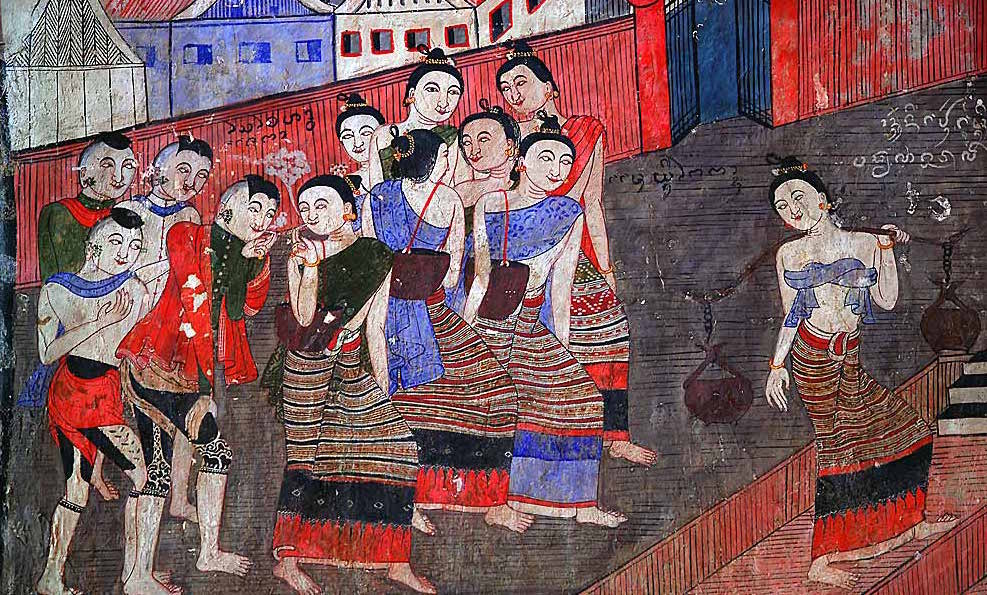
\includegraphics[width=0.6\linewidth]{images/show_peicewise/fig2a.jpg}
		\]
		\caption{ภาพจิตรกรรมไทยที่วัดภูมินทร์ อำเภอเมือง จังหวัดน่าน}
		\label{fig2}
	\end{figure}
	
	
	\subsection{การลบบทบรรยายบนอนิเมะ}
	\hspace{1cm}อนิเมะคือวิดีโอภาพวาดการ์ตูนสไตล์ญี่ปุ่นซึ่งเป็นที่นิยมของเยาวชนไทย ในการรับชมอนิเมะ แม้ว่าเยาวชนไทยสามารถรับชมด้วยบทพากย์เสียงภาษาไทย แต่ก็สูญเสียอรรถรสของการรับชมจากบทบรรยายแบบแข็ง\footnote{บทยรรยายที่ไม่สามารถปิดหรือเปิดได้} (hardsub) ที่เป็นภาษาต่างประเทศในบริเวณด้านล่างของจอภาพ ในการซ่อมแซม\\อนิเมะด้วยการลบบทบรรยายภาษาต่างประเทศจึงเป็นงานที่ยุ่งยากและท้าท้ายมาก เนื่องจาก
	\begin{itemize}
		\item [(1)] อนิเมะเป็นวิดีโอซึ่งแสดงผลประมาณ 24 เฟรม(ภาพ)ต่อวินาที
		\item [(2)] แต่ละเฟรมอาจมีหรืออาจไม่มีบทบรรยายก็ได้
		\item [(3)] แต่ละเฟรมอาจมีหรืออาจไม่มีบทบรรยายเดียวกันก็ได้
		\item [(4)] แต่ละเฟรมเป็นการแสดงผลภาพสีที่มีระดับความคมชัดสูง (high definition) ขนาดมากถึง $1920\times1080$ พิกเซล
	\end{itemize}
	ด้วยความท้าทายข้างต้น การพัฒนาขั้นตอนวิธีการต่อเติมภาพที่สามารถกำหนดโดเมนต่อเติมเชิงอัตโนมัติให้กับแต่ละเฟรมและประมวลผลได้แม่นยำจนการลบบทบรรยายสามารถทำงานได้แบบเรียลไทม์จึงเป็นสิ่งจำเป็นที่หลีกเลี่ยงไม่ได้
	
	\hspace{1cm} รูปที่ \ref{fig3} แสดงตัวอย่าง 1 เฟรมของอนิเมะที่มีบทบรรยายแบบแข็ง\footnote{ภาพจาก https://www.samehadaku.tv/2018/07/grand-blue-episode-1-subtitle-indonesia.html สืบค้นเมื่อวันที่ 23 กันยายน 2561} ที่ต้องซ่อมแซมด้วยการลบบทบรรยายออก  ทั้งนี้ในการลบบทบรรยายออกจากเฟรมโดยใช้การต่อเติมภาพ เราจะเริ่มด้วยการสร้างโดเมนต่อเติมแบบอัตโนมัติในบริเวณบทบรรยาย จากนั้นจึงนำขั้นตอนวิธีการต่อเติมภาพแบบเร็วเพื่อลบบทบรรยายออกจากเฟรม 
	
	\begin{figure}[h]
		\[
		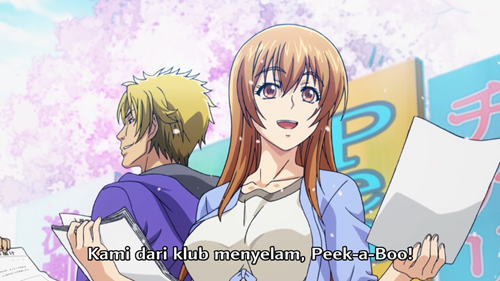
\includegraphics[width=0.6\linewidth]{images/show_peicewise/fig3.png}
		\]
		\caption{1 เฟรมของอนิเมะที่มีบทบรรยายแบบแข็ง}
		\label{fig3}
	\end{figure}
	
	\hspace{1cm} โครงการวิจัยนี้ ผู้วิจัยมีเป้าหมายสำคัญคือการพัฒนาขั้นตอนวิธีการต่อเติมภาพแบบเร็วและแม่นยำชนิดใหม่เพื่อนำไปใช้สำหรับซ่อมแซมภาพจิตรกรรมไทยและการลบบทบรรยายออกจากอนิเมะ


\section{วรรณกรรมและทฤษฎีบทที่เกี่ยวข้อง} 
\hspace{1cm} ในการกล่าวถึงขั้นตอนวิธีการต่อเติมภาพ จะเริ่มต้นด้วยการกล่าวทบทวนเกี่ยวกับการต่อเติมภาพเฉดสีเทา (grayscale image) ก่อน ดังนี้

\hspace{1cm} ให้ $\Omega \subset \mathbb{R}^2$ แทนโดเมนภาพ (image domain) $D \subset \mathbb{R}^2$ แทนโดเมนต่อเติม (ดูรูปที่ \ref{fig4}) และ $V \subset [0,\infty)$ 

\hspace{1cm} ให้ $ u: \Omega \rightarrow V,\ z: \Omega \rightarrow V$ แทนภาพที่ได้รับการซ่อมแซมและภาพที่ต้องการซ่อมแซม ตามลำดับ

\hspace{1cm} ในที่นี้ $ \mathbf{x} = (x,y) \in \Omega $ แทนพิกัดทางกายภาพ (physical position) ของภาพ และ $ u(\mathbf{x}) \in V $ แทนระดับความเข้มของภาพ (image intensity) ที่ $ \mathbf{x} $ และ $ \Omega $ มีรูปร่างสี่เหลี่ยม 

\hspace{1cm} นอกจากนี้เราสามารถสมมติได้โดยไม่เสียหลักการสำคัญว่า $ \Omega = [1,n]^2 $ และ $ V = [0,1] $ เมื่อ $n>0$ เป็นจำนวนเต็มบวก ทั้งนี้ เราจะเรียกภาพ $u,z$ ที่นิยามข้างต้นว่าภาพเฉดสีเทา
\begin{figure}[H]
	\centering
	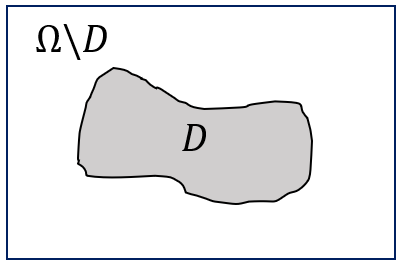
\includegraphics[width=0.4\linewidth]{images/sample-domain.png}
	\caption{$D$ แทนโดเมนต่อเติม}
	\label{fig4}
\end{figure}

\subsection{ตัวแบบการต่อเติมภาพเฉดสีเทาที่ใช้การแปรผันรวม}\label{inpaint-model-grayscale}

\hspace{1cm} ในการต่อเติมภาพเฉดสีเทา Chan และ Shen \cite{ref:rof-inpaint-chan-shen} ได้นำเสนอตัวแบบเชิงการแปรผัน (variational model) ที่ใช้เร็กกิวลาร์ไรซ์เซชันแบบการแปรผันรวม (Total variation based regularization) โดยพัฒนาต่อจากตัวแบบ ROF สำหรับการกำจัดสัญญาณรบกวน \cite{ref:ROF-template} ซึ่งตัวแบบเชิงการแปรผันนี้กำหนดโดย
\begin{align}
\min_{u} \{ \mathcal{J}(u) = \frac{1}{2} \int_{\Omega}\lambda (u-z)^2 d\Omega +  \int_{\Omega}  |\nabla u|  d\Omega \}
\label{e1}
\end{align}
เมื่อ 
\begin{align}
\lambda=\lambda(\mathbf{x}) = \left \{ \begin{array}{ll}  \lambda_0, & x \in \Omega \textbackslash D \\ 0, & x \in D  \end{array} \right . 
\label{e2}
\end{align}
แทนพารามิเตอร์เร็กกิวลาร์ไรซ์เซชัน (regularization parameter) และ $\lambda_0 >0$

\hspace{1cm} โดยแคลคูลัสของการแปรผัน (Calculus of variations) จะได้สมการออยเลอร์ลากรางจ์ที่เกี่ยวข้องกับ (\ref{e1}) เป็น 
\begin{align}
\left \{ \begin{array}{ll}  - \nabla \cdot  \Big( \dfrac{\nabla u}{|\nabla u|} \Big) + \lambda (u-z) = 0,  & \hspace{1cm} \mathbf{x} \in (1,n)^2 \\ \dfrac{\partial u}{\partial \boldsymbol{n}} = 0, & \hspace{1cm} x \in \partial \Omega \end{array} \right . 
\label{e3}
\end{align}
เมื่อ $\boldsymbol{n}$ แทนเวกเตอร์หน่วยที่ตั้งฉากกับของของภาพ

\hspace{1cm} ต่อไปจะกล่าวทบทวนวิธีการเชิงตัวเลขสำหรับแก้สมการเชิงอนุพันธ์ย่อยใน (\ref{e3}) 

\begin{itemize}
	\item [(1)] วิธีการเดินเวลาแบบชัดแจ้ง (explicit time marching method) 
	
	คณะวิจัย \cite{ref:ROF-template} ได้แนะนำวิธีการเชิงตัวเลขสำหรับการกำจัดสัญญาณรบกวนโดยใช้วิธีการเดินเวลาแบบชัดแจ้ง ซึ่งสามารถประยุกต์เป็นวิธีเชิงตัวเลขสำหรับการต่อเติมภาพได้ดังนี้
	
	\hspace{1cm} เริ่มจากการแนะนําตัวแปรเวลาสังเคราะห์ (time artificial variable) จากนั้นหาคําตอบแบบสภาวะคงตัว (steady-state solution) ในขณะที่ $t\rightarrow \infty$ ของสมการเชิงอนุพันธ์ย่อยไม่เป็นเชิงเส้นที่ขึ้นอยู่กับเวลา 
	\begin{align}
	u(\mathbf{x},t_{k+1})=u(\mathbf{x},t_{k})+\tau\left(\nabla \cdot\left(\dfrac{\nabla u (\mathbf{x},t_k)}{| \nabla u (\mathbf{x},t_k) | }\right) + \lambda(\mathbf{x})(u (\mathbf{x},t_k)-z(\mathbf{x})) \right),\ u(\mathbf{x},t_0)=z
	\label{e4}
	\end{align}
	เมื่อ $t_k=t_0+k\tau\ (\tau>0)$  แทนขั้นเวลาที่ $k$ และ $t_0=0$ แทนขั้นเวลาเริ่มต้น
	
	\item [(2)] วิธีการทำซ้ำแบบจุดตรึง (fixed-point iteration method)
	
	คณะวิจัย \cite{ref:FixpointSolver} ได้แนะนำวิธีการเชิงตัวเลขสำหรับการกำจัดสัญญาณรบกวนโดยใช้วิธีการทำซ้ำแบบจุดตรึง ซึ่งสามารถประยุกต์เป็นวิธีเชิงตัวเลขสำหรับการต่อเติมภาพได้ดังนี้
	
	\hspace{1cm} เริ่มจากการแนะนำดัชนีการทำซ้ำแบบจุดตรึง $\nu=0,1,2,\cdots$ และนิยามรูปแบบการทำซ้ำโดย
	\begin{align}
	- \nabla\cdot\left(\dfrac{\nabla u^{[\nu+1]}}{{| \nabla u |}^{[v]} }\right) + \lambda(u^{[\nu+1]}-z)  = 0,\ u^{[0]}=z
	\label{e5}
	\end{align}
\end{itemize}

\hspace{1cm} เนื่องจาก $\tfrac{1}{| \nabla u |}=\tfrac{1}{\sqrt{u_x^2+u_y^2}} \rightarrow \infty$ ในบริเวณที่ $u$ มีความเข้มสีเป็นเอกพันธ์ุ ($u(\mathbf{x})=$ ค่าคงตัว) เพื่อหลีกเลี่ยงปัญหาเชิงตัวเลขจะเกิดขึ้นใน (\ref{e4}) และ (\ref{e5}) เราจะใช้ 
\[
|\nabla u| \approx| \nabla u |_\beta=\sqrt{u_x^2+u_y^2+\beta},\ 0< \beta \ll 1
\] 

\hspace{1cm} จาก (\ref{e4}) และ (\ref{e5}) เราพบว่ายิ่ง $\beta$ มีค่าน้อยลงมากขึ้นเท่าไหร่ ความแม่นยำของตัวแบบ (\ref{e1}) ยิ่งมีมากขึ้นเท่านั้น นอกจากนี้ เรายังพบอีกว่า การแก้สมการ (\ref{e4}) และ (\ref{e5}) ยิ่งมีความยุ่งยากมากขึ้นสำหรับ $\beta$ ที่มีค่าน้อยๆ 

\hspace{1cm} เพื่อเอาชนะความยากเชิงตัวเลขนี้ คณะวิจัยโดย \cite{ref:splitbergman-inpaint} ได้แนะนำวิธีการสปริทเบรกแมนซึ่งสามารถกล่าวถึงพอสังเขป ดังนี้

\begin{itemize}
	\item [(3)] วิธีการสปริทเบรกแมน (Split Bregman method)
	
	เริ่มจากการแนะนำเวกเตอร์เสริม $\boldsymbol{w}$ พารามิเตอร์เบรกแมน (Bregman parameter) $\boldsymbol{b}$ และพารามิเตอร์เพนัลที (panalty parameter) $\theta>0$ และเขียน (\ref{e1}) ใหม่ ดังนี้
	\begin{align}
	\min_{u,\boldsymbol{w}} \{ \mathcal{J}(u,\boldsymbol{w}) = \dfrac{1}{2} \int_{\Omega} \lambda(u-z)^2 d\Omega +  \int_{\Omega}  |\nabla \boldsymbol{w}|  d\Omega + \frac{\theta}{2} \int_{\Omega} (\boldsymbol{w} - \nabla u + \boldsymbol{b}) d\Omega \}
	\label{e6}
	\end{align}
	สำหรับการหาคำตอบของ (\ref{e6}) เราจะใช้วิธีการหาค่าต่ำที่สุดแบบสลับ (alternating minimization method) โดยเริ่มจากการตรึง $\boldsymbol{w}^{\text{old}}$ และ $\boldsymbol{b}^{\text{old}}$ จากนั้นแก้ปัญหาย่อย
	\begin{align}
	u^{\text{New}}=\underset{u}{\arg\min} \{ \mathcal{J}_1(u) = \dfrac{1}{2} \int_{\Omega} \lambda(u-z)^2 d\Omega + \frac{\theta}{2} \int_{\Omega} (\boldsymbol{w}^{\text{old}} - \nabla u + \boldsymbol{b}^{\text{old}}) d\Omega \}
	\label{e7}
	\end{align}
	จากนั้นใช้ $u^{\text{New}}$ ที่ได้จากการแก้ปัญหาย่อยใน (\ref{e7}) เพื่อแก้ปัญหาย่อย
	\begin{align}
	\boldsymbol{w}^{\text{New}}=\underset{\boldsymbol{w}}{\arg\min} \{ \mathcal{J}_2(\boldsymbol{w}) = \int_{\Omega}  |\nabla \boldsymbol{w}|  d\Omega  + \frac{\theta}{2} \int_{\Omega} (\boldsymbol{w} - \nabla u^{\text{New}} + \boldsymbol{b}^{\text{old}}) d\Omega \}
	\label{e8}
	\end{align}
	สุดท้ายจึงปรับปรุงพารามิเตอร์เบรกแมน 
	\begin{align}
	\boldsymbol{b}^{\text{New}}=\boldsymbol{b}^{\text{old}}+\nabla u^{\text{New}}-\boldsymbol{w}^{\text{New}}
	\label{e9}
	\end{align}
	ดำเนินการเช่นนี้จนกระทั่ง $||u^{\text{new}}-u^{\text{old}}||< \epsilon_1$ หรือ $\text{New}>\epsilon_2$ เมื่อ $\epsilon_1,\epsilon_2>0$ 
\end{itemize}

\subsection{ตัวแบบการต่อเติมภาพสีที่ใช้การแปรผันรวม}\label{inpaint-model-color}

\hspace{1cm} ต่อไปเราจะพิจารณาภาพสีในระบบ RGB นั่นคือ เราสมมติว่า

$$ \boldsymbol{u} = (u_1,u_2,u_3)^{\top},\ \boldsymbol{z} = (z_1,z_2,z_3)^{\top} : \Omega  \rightarrow V^3 $$

\noindent เมื่อ $u_1,u_2,u_3: \Omega  \rightarrow V$ และ $z_1,z_2,z_3: \Omega  \rightarrow V$ แทนภาพในเฉดสีแดง สีเขียว และสีน้ำเงินของ $\boldsymbol{u},\boldsymbol{z}$ ตามลำดับ 

\hspace{1cm} ในทำนองเดียวกันกับตัวแบบการต่อเติมภาพเฉดสีเทาที่ใช้การแปรผันรวม ตัวแบบการต่อเติมภาพสีที่ใช้การแปรผันรวมสามารถเขียนได้ดังนี้
\begin{align}
\min_{\boldsymbol{u}} \{ \bar{\mathcal{J}}(\boldsymbol{u})= \mathcal{\bar{D}}(\boldsymbol{u},\boldsymbol{z})+  \mathcal{\bar{R}}(\boldsymbol{u}) \}
\label{e10}
\end{align}
เมื่อ
\begin{align*}
\mathcal{\bar{D}}(\boldsymbol{u},\boldsymbol{z}) 
&= \frac{1}{2}\int_{\Omega}^{}\lambda(u_1 - z_1)^2 d\Omega + \frac{1}{2}\int_{\Omega}^{}\lambda(u_2 - z_2)^2 d\Omega + \frac{1}{2}\int_{\Omega}^{}\lambda(u_3 - z_3)^2 d\Omega
\end{align*}
และ 
\begin{align*}
\mathcal{\bar{R}}(\boldsymbol{u})= \int_{\Omega}^{}\lvert\nabla u_1 \rvert d\Omega + \int_{\Omega}^{}\lvert\nabla u_2 \rvert d\Omega + \int_{\Omega}^{}\lvert\nabla u_3 \rvert d\Omega
\end{align*}

\hspace{1cm} เพื่อหลีกเลี่ยงปัญหาที่มาจากเทอม $\tfrac{1}{|\nabla u_l|}\ (l=1,2,3)$ โครงงานวิจัยนี้จะพัฒนาขั้นตอนวิธีเชิงตัวเลขสำหรับต่อเติมภาพจากวิธีการสปริทเบรกแมน
โดยแก้ปัญหาการหาค่าต่ำที่สุดต่อไปนี้
\begin{align}
\min_{\boldsymbol{u},\boldsymbol{w}_1,\boldsymbol{w}_2,\boldsymbol{w}_3} \{\bar{\mathcal{J}}(\boldsymbol{u},\boldsymbol{w}_1,\boldsymbol{w}_2,\boldsymbol{w}_3)&= \mathcal{\bar{D}}(\boldsymbol{u},\boldsymbol{z}) +  \underset{l=1}{\overset{3}{\sum}} \int_{\Omega}^{}|\boldsymbol{w}_l|d\Omega
\nonumber\\
&\quad+ \frac{\theta_l}{2} \underset{l=1}{\overset{3}{\sum}}\int_{\Omega}^{}(\boldsymbol{w}_l - \nabla u_l - \boldsymbol{b_l})^{2}d\Omega\}, \hspace{1cm} \theta_l > 0
\end{align}
ด้วยวิธีการหาต่ำที่สุดแบบสลับดังเช่น (\ref{e6}) - (\ref{e9})

\section{ผลการดำเนินงานเบื้องต้น}
	\subsection{การซ่อมแซมภาพจิตรกรรมไทยโบราณ}
	\hspace{1cm} สำหรับการซ่อมแซมจิตรกรรมไทยโบราณ ก่อนอื่นจะทำการปรับปุรงขั้นตอนวิธีเชิงตัวเลขที่มีอยู่แต่เดิมก่อน โดยระหว่างการปรับปรุงวิธีเชิงตัวเลข จะใช้ภาพที่ได้สร้างขึ้น 5 ภาพ แต่ละภาพมีขนาด 256 x 256 พิกเซล ซึ่งมีดังนี้
	\begin{figure}[H]
		\centering
		\begin{subfigure}{0.15\linewidth}
			\centering
			
\includegraphics[width=0.8\linewidth]{images/image_inpaint_synthetic/case01-original.png}
		\end{subfigure}
		\begin{subfigure}{0.15\linewidth}
			\centering
			
\includegraphics[width=0.8\linewidth]{images/image_inpaint_synthetic/case02-original.png}
		\end{subfigure}
		\begin{subfigure}{0.15\linewidth}
			\centering
			
\includegraphics[width=0.8\linewidth]{images/image_inpaint_synthetic/case03-original.png}			
		\end{subfigure}
		\begin{subfigure}{0.15\linewidth}
			\centering
			
\includegraphics[width=0.8\linewidth]{images/image_inpaint_synthetic/case04-original.png}			
		\end{subfigure}
		\begin{subfigure}{0.15\linewidth}
			\centering
			
\includegraphics[width=0.8\linewidth]{images/image_inpaint_synthetic/case05-original.png}			
		\end{subfigure}
		\caption{ภาพต้นฉบับ}
	\end{figure}
	\begin{figure}[H]
		\centering
		\begin{subfigure}{0.15\linewidth}
			\centering
			
\includegraphics[width=0.8\linewidth]{images/image_inpaint_synthetic/case01-toinpaint.png}
		\end{subfigure}
		\begin{subfigure}{0.15\linewidth}
			\centering
			
\includegraphics[width=0.8\linewidth]{images/image_inpaint_synthetic/case02-toinpaint.png}
		\end{subfigure}
		\begin{subfigure}{0.15\linewidth}
			\centering
			
\includegraphics[width=0.8\linewidth]{images/image_inpaint_synthetic/case03-toinpaint.png}			
		\end{subfigure}
		\begin{subfigure}{0.15\linewidth}
			\centering
			
\includegraphics[width=0.8\linewidth]{images/image_inpaint_synthetic/case04-toinpaint.png}			
		\end{subfigure}
		\begin{subfigure}{0.15\linewidth}
			\centering
			
\includegraphics[width=0.8\linewidth]{images/image_inpaint_synthetic/case05-toinpaint.png}			
		\end{subfigure}
		\caption{ภาพที่จะทำการซ่อมแซม}
	\end{figure}
	\subsubsection{การเปรียบเทียบประสิทธิภาพขั้นตอนวิธีเชิงตัวเลขที่มีอยู่สำหรับตัวแบบต่อเติมภาพสีที่ใช้การแปรผันรวม}
	
	\hspace{1cm} โดยจะทำการเปรียบเทียบความเร็วของวิธีการแก้การแปรผันรวมที่มีอยู่เดิม ดังที่ได้กล่าวไว้ในหัวข้อ \ref{inpaint-model-grayscale} และหัวข้อ \ref{inpaint-model-color} โดยวิธีการทั้ง 3 วิธี จะทำการทำซ้ำจนกระทั่งภาพในการทำซ้ำรอบปัจจุบัน กับภาพการทำซ้ำในครั้งก่อนหน้า มีค่าความคลาดเคลื่อนสัมพัทธ์ (relative error) ต่างกันไม่เกิน 0.0001 หรือ ทำซ้ำเกิน 10,000 รอบ ซึ่งได้ผลลัพธ์เฉลี่ยของรูปภาพที่ใช้ทดสอบดังนี้

	\begin{table}[H]
		\centering
		\begin{tabular}[ht]{|l|c|c|c|c|}
			\hline
			วิธีการ  & เวลาประมวล  (วินาที) & PSNR (dB) & SSIM \\
			\hline
			การเดินเวลา & 146.2108 & 16.19756 & 0.9954786\\
			การทำซ้ำจุดตรึง & 72.32298 & 40.12234 & 0.999905\\
			การสปริทเบิร์กแมน & 11.438246 & 39.39536 & 0.999894 \\
			\hline
		\end{tabular}
		\caption{แสดงผลลัพธ์เฉลี่ยของวิธีการเชิงตัวเลขสำหรับการต่อเติมภาพ}
	\end{table}	
	\hspace{1cm} จะเห็นว่าจากตาราง พบว่าแม้วิธีการทำซ้ำจุดตรึง และวิธีการสปริทเบรกแมน จะมีคุณภาพใกล้เคียงกัน แต่ว่าวิธีการสปริทเบรกแมน ใช้เวลาในการประมวลผลน้อยกว่ามาก ผู้วิจัย จึงนำวิธีการสปริทเบรกเมนไปใช้พัฒนาวิธีการต่อเติมภาพชนิดใหม่ลำดับถัดไป
	
	\subsubsection{ขั้นตอนวิธีการสำหรับต่อเติมภาพชนิดใหม่}
	\hspace{1cm} จากวิธีการสปริทเบรกแมนนั้นจะใช้วิธีการหาคำตอบโดยวิธีการทำซ้ำจนกระทั่งลู่เข้า ทางผู้ศึกษาจึงสนใจที่หาคำตอบเริ่มต้นสำหรับการทำซ้ำที่ดีขึ้น เพื่อทำให้การทำซ้ำลู่เข้าสู่คำตอบได้เร็วขึ้น โดยการทำงานกับรูปภาพที่เล็กกว่า จากนั้นจึงทำการขยายลัพธ์ที่ได้ขึ้นมาทำกับภาพใหญ่ ซึ่งวิธีนี้เรียกว่าวิธีพีระมิดรูปภาพ ( pyramid methods) \cite{ref:image-pyramid}  โดยผู้วิจัยจะทำการย่อขนาดรูปลงครึ่งนึงโดยใช้วิธี Bilinear Interpolation ทั้งสิ้น 4 ครั้ง จากนั้นเริ่มทำการต่อเติมภาพขนาดเล็ก จากนั้นนำผลลัพธ์ที่ได้จากภาพขนาดเล็ก ทำการขยายภาพขึ้นสองเท่าโดยใช้ Bilinear Interpolation
	 ก่อนจะนำเฉพาะส่วนที่อยู่ในโดเมนต่อเติมของภาพที่ถูกขยายมาทำการต่อเติมเพื่อให้ส่วนที่ถูกขยายขึ้นมาเป็นคำตอบเริ่มต้นสำหรับการต่อเติมภาพในขั้นที่สูงขึ้น
	 
	 	\begin{figure}[H]
	 	\centering
	 	\begin{subfigure}{0.4\linewidth}
	 		\centering
	 		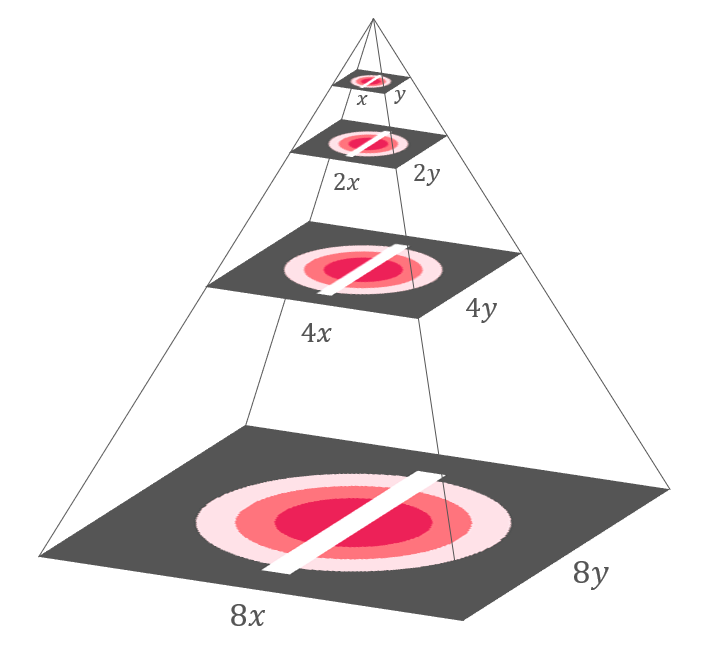
\includegraphics[width=0.8\linewidth]{images/image_inpaint_synthetic/image_pyramid.png}
	 	\end{subfigure}
 		 \caption{วิธีการพีระมิดรูปภาพ}
	 \end{figure}
 	\hspace{1cm} อย่างเช่นภาพที่ \ref{image:intialsolution} จากภาพที่ต้องการซ่อมแซมทางด้านซ้าย จะทำการย่อภาพให้เหลือขนาดเล็กเพื่อจะได้ทำการต่อเติมภาพได้อย่างรวดเร็ว หลังจากนั้นเมื่อทำการต่อเติมภาพขนาดเล็กเสร็จแล้ว จะทำการขยายภาพขึ้นแล้วทำการนำพื้นทีี่จากภาพที่ขยายขึ้นไปแทนในโดเมนต่อเติมแล้ว จะได้ภาพนั้น ในส่วนที่เป็นโดเมนต่อเติมจะมีลักษณะเบลอ แต่มีสีใกล้เคียงกับคำตอบที่ต้องการ  ซึ่งหลังจากนี้จะนำภาพทางด้านขวาไปทำการต่อเติมจนได้คำตอบที่ต้องการ โดยเมื่อใช้สีที่เบลอแต่มีใกล้เคียงเป็นคำตอบเริ่มต้นที่ใช้เวลาการประมวลผลน้อยกว่าการนำภาพไปต่อเติมโดยไม่ผ่านการใช้พีระมิด
	 \begin{figure}[H]
	 	\centering
	 	\begin{subfigure}{1\linewidth}
	 		\centering
	 		
\includegraphics[width=0.8\linewidth]{images/image_inpaint_synthetic/image_inital_solution.png}
	 	\end{subfigure}
	 	\caption{การเตรียมคำตอบเริ่มต้นจากภาพขนาดเล็ก}
	 	\label{image:intialsolution}
	 \end{figure}
	
	\hspace{1cm} โดยจะทำการเปรียบเทียบจำนวนครั้งในชั้นที่รูปภาพมีขนาดเล็ก จนไปถึงชั้นที่มีขนาดใหญ่ ตัวอย่าง เช่น 10/3/3/10000 หมายถึงในชั้นเล็กสุดซึ่งขนาดเป็น 32x32 พิกเซลจะทำซ้ำ 10 ครั้งหรือจนค่าความคลาดเคลื่อนสัมพัทธ์ต่างกันไม่เกิน 0.0001  ชั้นถัดมาขนาดเป็น 64x64 จะทำซ้ำ 3 ครั้งหรือจนค่าความคลาดเคลื่อนสัมพัทธ์ต่างกันไม่เกิน 0.0001 และชั้นถัดมา ชั้นถัดมาขนาดเป็น 128x128 จะทำซ้ำ 3 ครั้งหรือจนค่าความคลาดเคลื่อนสัมพัทธ์ต่างกันไม่เกิน 0.0001 และสุดท้ายขนาด 256x256 จะทำซ้ำ 3 ครั้งหรือจนค่าความคลาดเคลื่อนสัมพัทธ์ต่างกันไม่เกิน 0.0001 ซึ่งเมื่อทำการทดสอบแล้วได้ผลลัพธ์ดังตารางนี้
	
		\begin{table}[H]
		\centering
		\begin{tabular}[ht]{|l|c|c|c|c|}
			\hline
			รูปแบบการทำซ้ำ  & เวลาประมวล  (วินาที) & PSNR (dB) & SSIM \\
			\hline
			ไม่ใช้พีระมิดรูปภาพ & 13.690378 & 30.72924 & 0.9997676 \\
			10/1/1/10000 & 8.719006 & 30.5632 & 0.9997186 \\
			10/3/3/10000 & 5.8064316 & 30.62492 & 0.9997298 \\
			10/10/10/10000 & 2.6100824 & 30.64522 & 0.9997388 \\
			100/1/1/10000 & 5.839534 & 30.68802 & 0.9997514 \\
			100/3/3/10000 & 4.4923898 & 30.68914 & 0.9997498 \\
			100/10/10/10000 & 2.4151272 & 30.67366 & 0.9997476 \\
			\hline
		\end{tabular}
		\caption{แสดงผลลัพธ์เฉลี่ยของการใช้พีระมิดภาพในการต่อเติมในชั้นที่ต่างกัน}
	\end{table}	
	
	จากตารางจะสังเกตว่า ยิ่งจำนวนการทำซ้ำในชั้นที่รูปภาพมีขนาดเล็กจำนวนมาก ยิ่งประมวลผลได้เร็วขึ้น 
	
	นอกจากนี้แล้ว ผู้วิจัยยังได้สังเกตอีกว่า การทำซ้ำนั้น จะลู่เข้าเร็วในช่วงแรก จากนั้นความเร็วในการลู่เข้าจะลดลง ซึ่งทำให้การทำซ้ำเพียงไม่กี่ครั้งในรูปภาพขนาดใหญ่สุด มีผลลัพธ์ใกล้เคียงกับภาพต้นฉบับได้
	
	\begin{figure}[H]
		\centering
		\begin{subfigure}{0.23\linewidth}
			\centering
			
\includegraphics[width=0.8\linewidth]{images/just10enough/only10time.png}
			\caption{ชั้นใหญ่สุด 10 ครั้ง}
		\end{subfigure}
		\begin{subfigure}{0.23\linewidth}
			\centering
			
\includegraphics[width=0.8\linewidth]{images/just10enough/only100time.png}
			\caption{ชั้นใหญ่สุด 100 ครั้ง}
		\end{subfigure}
		\begin{subfigure}{0.23\linewidth}
			\centering
			
\includegraphics[width=0.8\linewidth]{images/just10enough/only1000time.png}			
			\caption{ชั้นใหญ่สุด 1,000 ครั้ง}
		\end{subfigure}
		\begin{subfigure}{0.23\linewidth}
			\centering
			
\includegraphics[width=0.8\linewidth]{images/just10enough/only10000time.png}			
			\caption{ชั้นใหญ่สุด 10,000 ครั้ง}
		\end{subfigure}
		\caption{พีระมิดที่ลำดับการทำซ้ำเป็น 10/10/10 และชั้นใหญ่สุดทำในจำนวนครั้งที่ต่างกัน}
	\end{figure}
	
	 โดยผู้วิจัยจึงกำหนดให้การทำซ้ำในรูปภาพขนาดใหญ่สุดมีการทำซ้ำเพียง 10 ครั้ง และพบว่าได้ผลลัพธ์ดังนี้
	
	\begin{table}[H]
		\centering
		\begin{tabular}[ht]{|l|c|c|c|c|}
			\hline
			รูปแบบการทำซ้ำ  & เวลาประมวล  (วินาที) & PSNR (dB) & SSIM \\
			\hline
			ไม่ใช้พีระมิดรูปภาพ & 0.394235 & 25.22906 & 0.9989972 \\
			10/1/1/10 & 0.3839476 & 31.31306 & 0.9997732 \\
			10/3/3/10 & 0.3672704 & 30.95474 & 0.9997682 \\
			10/10/10/10 & 0.4077878 & 30.78114 & 0.9997406 \\
			100/1/1/10 & 0.3789076 & 31.25708 & 0.9997518 \\
			100/3/3/10 & 0.3939378 & 30.8896 & 0.999746 \\
			100/10/10/10 & 0.4507862 & 30.81302 & 0.9997504 \\
			\hline
		\end{tabular}
		\caption{แสดงผลลัพธ์เฉลี่ยของการใช้พีระมิดภาพในการต่อเติมโดยกำหนดให้ชั้นรูปภาพขนาดใหญ่สุดทำซ้ำเพียง 10 ครั้ง}
	\end{table}	

	จากตารางจะเห็นว่า การทำซ้ำในชั้นที่รูปภาพมีขนาดเล็กมากจำนวนมาก ไม่ช่วยให้การประมวลผลได้เร็วขึ้น ผู้วิจัยจึงเลือกใช้การทำซ้ำแบบ 10/3/3/10 ในการต่อเติมภาพ
	
	\subsubsection{การทดสอบประสิทธิภาพในการซ่อมแซมภาพจิตรกรรมไทยโบราณ}
	\hspace{1cm}ซึ่งภาพจิตรกรรมทีี่ใช้ทดสอบ มีทั้งสิ้น 5  ภาพได้แก่ ภาพที่ 1 และภาพที่ 2 คือ จิตรกรรมฝาผนังวัดแก้วไพฑูรย์ ภาพที่ 3 คือ จิตรกรรมฝาผนังวัดพระยืนพุทธบาทยุคล ภาพที่ 4 คือ จิตรกรรมฝาผนังวัดคงคาราม และภาพที่ 5 คือ จิตรกรรมฝาผนังวัดท่าถนน
	โดยจะทำให้ข้อมูลข้องทั้ง 5 ภาพเกิดความเสียหาย โดยใช้รอยความเสียหายจากภาพพระเจ้าสร้างอดัม
	
	\begin{figure}[H]
		\centering
		\begin{subfigure}{0.25\linewidth}
			\centering
			
\includegraphics[width=0.7\linewidth]{images/thaiart/case01-original.png}
			\caption{วัดแก้วไพฑูรย์}
		\end{subfigure}
		\begin{subfigure}{0.25\linewidth}
			\centering
			
\includegraphics[width=0.7\linewidth]{images/thaiart/case02-original.png}
			\caption{วัดแก้วไพฑูรย์}
		\end{subfigure}
		\begin{subfigure}{0.25\linewidth}
			\centering
			
\includegraphics[width=0.7\linewidth]{images/thaiart/case03-original.png}
			\caption{วัดพระยืนพุทธบาทยุคล}
		\end{subfigure}

		\bigskip
		
		\begin{subfigure}{0.2\linewidth}
			\centering
			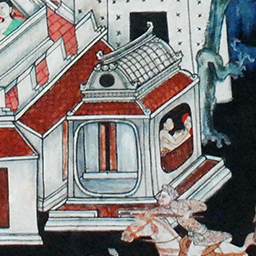
\includegraphics[width=0.8\linewidth]{images/thaiart/case04-original.png}
			\caption{วัดคงคาราม}
		\end{subfigure}
		\begin{subfigure}{0.2\linewidth}
			\centering
			
\includegraphics[width=0.8\linewidth]{images/thaiart/case05-original.png}
			\caption{วัดท่าถนน}
		\end{subfigure}
		\begin{subfigure}{0.2\linewidth}
			\centering
			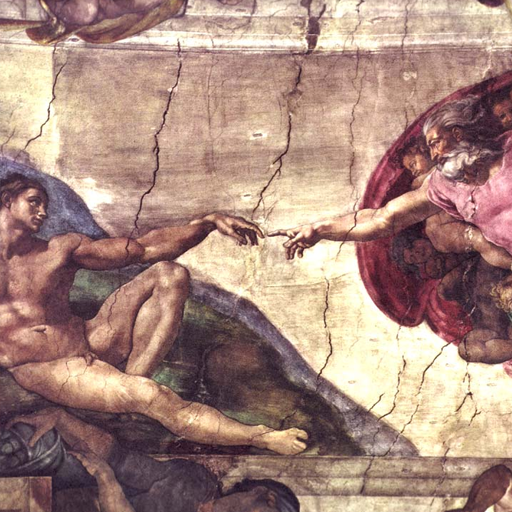
\includegraphics[width=0.8\linewidth]{images/thaiart/Restoration_of_the_Sistine_Chapel_frescoes.png}
			\caption{พระเจ้าสร้างอดัม}
		\end{subfigure}
		\begin{subfigure}{0.2\linewidth}
			\centering
			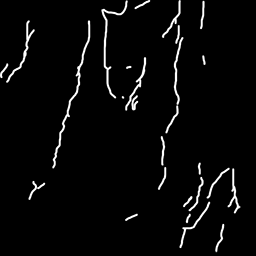
\includegraphics[width=0.8\linewidth]{images/thaiart/inpaint-domain.png}
			\caption{รอยความเสียหาย}
		\end{subfigure}
	\end{figure}
	
	 \hspace{1cm}  จากนั้นทำการทดสอบการต่อเติมภาพทั้ง 5 โดยทดสอบวิธีสปริทเบรกแมน วิธีทีที่พัฒนาขึ้นโดยใช้วิธีการสปริทเบรกแมนพร้อมทั้งการใช้พีระมิดรูปภาพที่มีการทำซ้ำแต่ละชั้นเป็น 10/3/3/10 และวิธี Fast Marching Method ซึ่งถูกเขีียนไว้ในชุดคำสั่ง OpenCV ได้ผลลัพธ์ออกเป็นดังตารางนี้

	\begin{table}[H]
		\centering
		\begin{tabular}[ht]{|l|c|c|c|c|}
			\hline
			วิธีการ  & เวลาประมวล  (วินาที) & PSNR (dB) & SSIM \\
			\hline
			สปริทเบรกแมน & 0.9518894 & 36.8499 & 0.9999882 \\ 
			วิธีการที่พัฒนาขึ้น & 0.2826256 & 36.79616 & 0.999988 \\
			OpenCV - Fast Marching Method & 0.0198226 & 35.56518 & 0.9968536 \\
			\hline
		\end{tabular}
		\caption{แสดงผลลัพธ์เฉลี่ยของการซ่อมแซมภาพศิลปะไทย}
	\end{table}	
	\hspace{1cm} ซึ่งจากตารางจะเห็นได้ว่า วิธีสปริทเบรกแมน นั้นแม้จะมี PSNR ทีดีกว่าเพียงเล็กน้อย แต่ SSIM กลับแย่กว่า และยังใช้เวลามากกว่าถึง 3 เท่า ส่วนวิธีการ Fast Marching Method แม้ว่าจะมีคุณภาพที่ด้อยกว่า ทั้งค่า PSNR และ SSIM แต่กลับมีเวลาที่รวดเร็วกว่ามาก
	
	
	
	\subsection{การลบบทบรรยายบนอนิเมะ}
	\hspace{1cm} สำหรับการลบบทบรรยายอนิเมะ จะใช้วิดีโอ Anime Festival Asia Special Video - feat. Inori Aizawa ซึ่งผลิตโดย Collateral Damage Studios โดยจะตัดวิดีโอ 1 นาทีแรกสำหรับการทดลอง โดยวิดีโอดังกล่าวขนาด 1280 x 720 พิกเซล แต่เนื่องจากโดยปกติแล้ว อนิเมะมักมีบรรทัดเพียง 1 ถึง 2 บรรทัด จึงทำการแบ่งวิดีโอออกอีกเป็น 5 ส่วนได้ขนาดเป็น 1280 x 144 พิกเซลก่อนนำไปทดสอบในลำดับถัดไป
	\hspace{1cm} และสำหรับบทบรรยายที่จะใช้ทดสอบนั้น เนื่องจากวิดีโอ Anime Festival Asia Special Video - feat. Inori Aizawa ไม่มีคำพูดใดๆ จึงใช้บทความ lorem ipsum เป็นบทบรรยาย โดยจะทำการแสดงบทบรรยาย 1 บรรทัด ความยาว 3 วินาที ทุก 2 วินาที นั่นคือในวิดีโอดังกล่าวจะมีบทบรรยายทั้งสิ้น 20 บรรทัด	
	
	\begin{figure}[H]
		\centering
		\begin{subfigure}{0.8\linewidth}
			\centering
			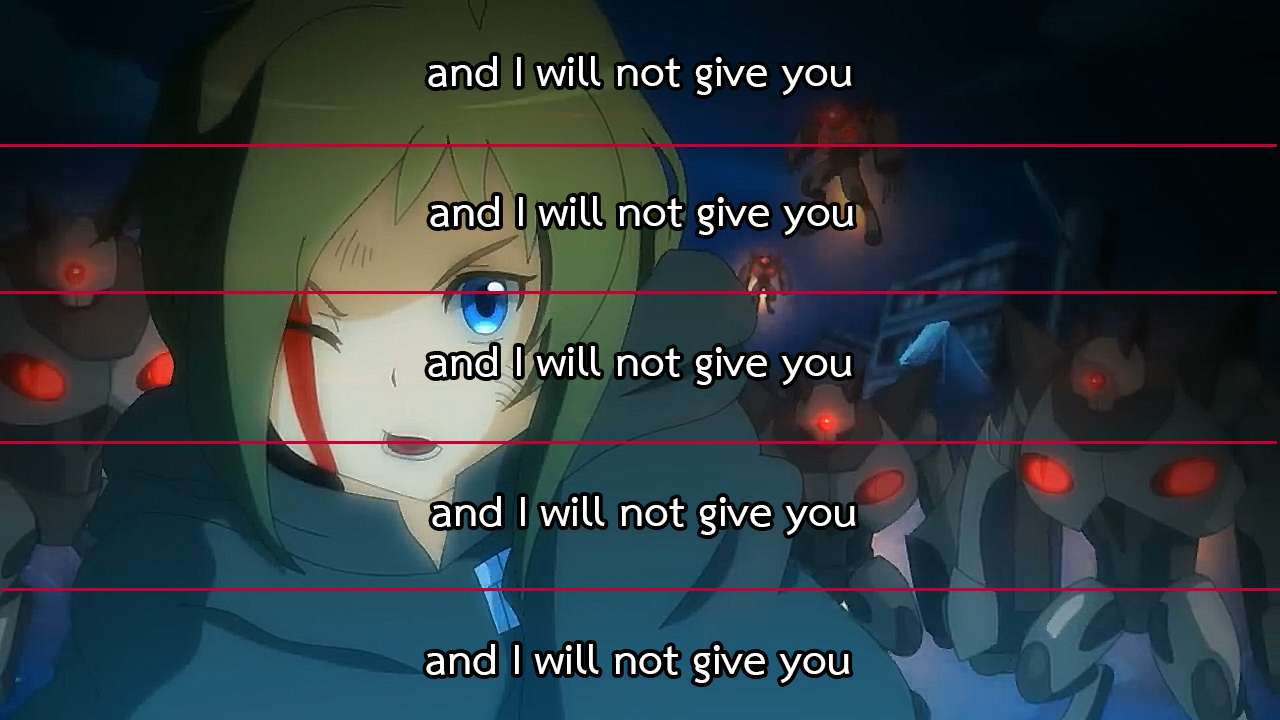
\includegraphics[width=0.8\linewidth]{images/inori-subbed-preview.png}
		\end{subfigure}
		\caption{การแบ่งไฟล์วิดีโอเป็น 5 ส่วนสำหรับใช้เป็น 5 ชุดทดสอบ}
	\end{figure}
	
	\subsubsection{การหาบทบรรยายบนอนิเมะ}	
	\hspace{1cm}ก่อนจะลบบทบรรยายนั้น จะเป็นต้องหาบทบรรยายในภาพให้ได้เสียก่อน โดยบทบรรยายของอนิเมะนั้น มักจะขึ้นบริเวณด้านล่างของหน้าจอ และนอกจากนี้ บทบรรยายอนิเมะมักจะใช้ขอบของตัวอักษรเป็นสีดำอีกด้วย ด้วยสมบัตินี้เองทำให้เราสามารถหาบริเวณบนเฟรมที่เป็นบทบรรยายได้โดยจะมีวิธีหาพื้นที่ซึ่งเป็นบทบรรยายดังนี้
	
	\begin{figure}[H]
		\begin{subfigure}{0.4\linewidth}
			\centering
			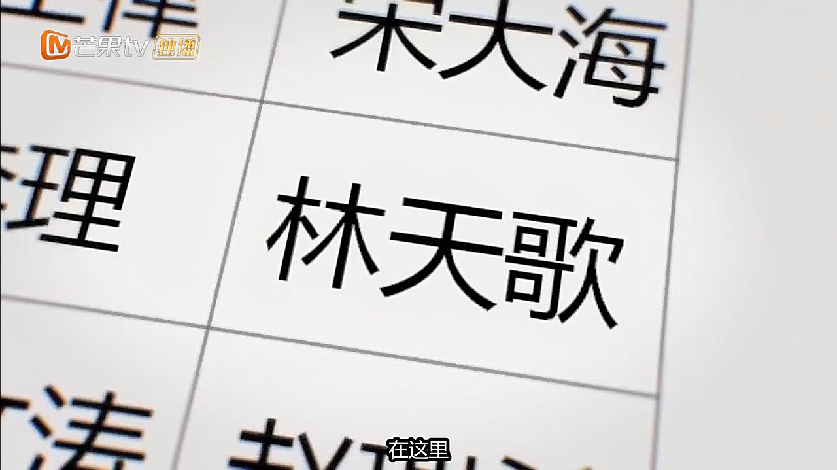
\includegraphics[width=0.8\linewidth]{images/subtitle_detection/detection-original.png}
			\caption{ภาพเฟรมอนิเมะบริเวณที่มีบทบรรยาย}
		\end{subfigure}
		\begin{subfigure}{0.4\linewidth}
			\centering
			
\includegraphics[width=0.8\linewidth]{images/subtitle_detection/detection-threshold.png}
			\caption{ภาพหลังทำการ thresholding}
		\end{subfigure}
	\end{figure}
	
	\hspace{1cm} ตัดเฟรมมาเฉพาะส่วนล่างของเฟรมที่น่าจะมีบทบรรยายปรากฏอยู่ จากนั้นทำการ thresholding เพื่อหาบริเวณที่เป็นสีดำเนื่องจากบทบรรยายจะถูกล้อมรอบด้วยสีดำเสมอ
	
	\begin{figure}[H]
		\begin{subfigure}{0.4\linewidth}
			\centering
			
\includegraphics[width=0.8\linewidth]{images/subtitle_detection/detection-inverse.png}
			\caption{ภาพหลังทำการสลับสีี}
		\end{subfigure}
		\begin{subfigure}{0.4\linewidth}
			\centering
			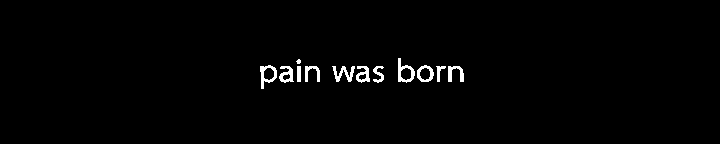
\includegraphics[width=0.8\linewidth]{images/subtitle_detection/detection-blackfill.png}
			\caption{ภาพหลังทำการเปลี่ยนพื้นที่สีขาว}
		\end{subfigure}
	\end{figure}
	
\hspace{1cm} 	ทำการสลับสีระหว่างสีดำกับสีขาวของภาพที่ทำการ thresholding หลังจากนั้นทำการเปลี่ยนพื้นที่สีขาวซึ่งติดกับขอบของเฟรมทั้งหมดให้เป็นสีดำ เพราะว่า บทบรรยายไม่อยู่ติดกับหน้าจอ เราจะถือว่าสิ่งที่อยู่ติดกับหน้าจอไม่ใช่บทบรรยาย
	
	\begin{figure}[H]
		\begin{subfigure}{0.4\linewidth}
			\centering
			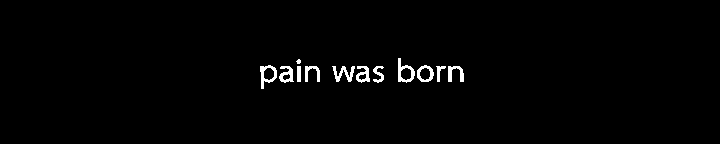
\includegraphics[width=0.8\linewidth]{images/subtitle_detection/detection-erode-opening.png}
			\caption{ภาพหลังการ erode และ opening}
		\end{subfigure}
		\begin{subfigure}{0.4\linewidth}
			\centering
			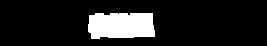
\includegraphics[width=0.8\linewidth]{images/subtitle_detection/detection-stoke.png}
			\caption{ภาพหลังการ dilate}
		\end{subfigure}
	\end{figure}
	
	\hspace{1cm} จากนั้นนำวัตถุที่มีขนาดเล็กเกินไป หรือใหญ่เกินไปออกจากภาพด้วยวิธีการ erode และ opening
	จะได้ว่าส่วนที่เหลือเป็นสีขาวในภาพคือบทบรรยาย แต่ว่าขอบของบทบรรยายก็ต้องถูกลบออกไปด้วย จึงทำการ dilate เพื่อขยายขอบของบทบรรยายให้เท่ากับบทบรรยายที่อยู่ในเฟรมวิดีโอ และสิ่งที่เหลืออยู่คือโดเมนต่อเติมที่จะนำไปใช้ในการซ่อมแซมภาพต่อไป
	
	\hspace{1cm} ซึ่งวิธีการหาบทบรรยายที่กล่าวไปข้างต้น จะทำการทดสอบกับบทความ lorem ipsum ที่ถูกแปลเป็นภาษาไทย ภาษาอังกฤษ และภาษาญี่ปุ่น โดยมีความสามารถในการหาโดเมนต่อเติมใบบทบรรยายภาษาต่างๆ  เฉลี่ยดังนี้
	
	\begin{table}[H]
		\centering
		\begin{tabular}[ht]{|l|c|c|c|c|}
			\hline
			ภาษา  & จำนวนพิกเซลในโดเมน & จำนวนพิกเซลที่ตรวจพบ & จำนวนพิกเซลที่ผิดพลาด & ร้อยละการผิดพลาด \\
			\hline
			ไทย & 23222219.8 & 24083124.8 & 2141201 & 9.220398882 \\
			อังกฤษ & 27278744.8 & 28598424.2 & 3714320.8 & 13.61613769 \\
			ญี่ปุ่น & 28544173 & 30103466.2 & 3740970.6 & 13.10584872 \\
			\hline
		\end{tabular}
		\caption{แสดงความคาดเคลื่อนเฉลี่ยของการหาโดเมนต่อเติม ในบทบรรยายภาษาต่างๆ}
	\end{table}	
	
	\hspace{1cm} จากการทดลองทั้ง  3 ภาษาพบว่าวิธีการหาคำบรรยายนี้ มีร้อยละการผิดพลาดเฉลี่ยอยู่ที่ 11.98 ซึ่งการทดลองจากนี้ไปจะใช้วิธีการหาคำบรรยายนี้ในการหาโดเมนต่อเติมแบบอัตโนมัติ
	
	\subsubsection{การลบคำบรรยายจากบทอนิเมะ}
	\hspace{1cm} สำหรับอนิเมะนั้น แต่ละเฟรมจะเป็นรูปภาพ เราจึงสามารถประยุกต์ใช้วิธีการซ่อมแซมภาพจิตรกรรมไทย มาใช้ในการลบคำบรรยายได้ แต่ผู้วิจัยก็ได้สังเกตว่า สำหรับอนิเมะที่เป็นวิดีโอแล้ว ในขณะที่ประมวลผลวิดีโอ เราสามารถใช้ผลการต่อเติมภาพจากภาพที่แล้ว มาใช้เป็นคำตอบเริ่มต้น โดยจะขอเรียกวิธีทั้งสองวิธีที่คิดขึ้นว่า วิธียืมเฟรม และวิธีข้ามเฟรม สำหรับวิธียืมเฟรม หากเฟรมก่อนหน้า กับเฟรมปัจจุบัน ในส่วนที่อยู่นอกโดเมนต่อเติม มีค่า SSIM มากกว่า 0.9 จะทำการใช้เฟรมก่อนหน้าเป็นค่าเริ่มต้นในการทำซ้ำแทนที่จะใช้ภาพที่มีคำบรรยายในการต่อเติม โดยจะนำส่วนที่อยู่ในโดเมนต่อเติมมาจากภาพก่อนหน้า ก่อนจะเริ่มการทำซ้ำเพื่อต่อเติมภาพ และวิธีข้ามเฟรมนั้น เมื่อบริเวณนอกโดเมนต่อเติมของเฟรมปัจจุบันกับเฟรมก่อนหน้า มีค่า SSIM มากกว่า 0.95 จะทำการคัดลอกบริเวณในโดเมนต่อเติมของภาพก่อนหน้ามาและข้ามไปประมวลผลเฟรมถัดไปทันที เพื่อลดเวลาการทำงาน 
	
	\begin{figure}[H]
		\centering
		\begin{subfigure}{0.4\linewidth}
			\centering
			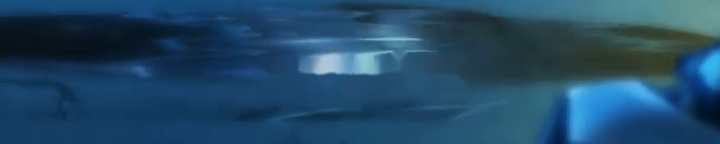
\includegraphics[width=0.8\linewidth]{images/skipborrow/prevframe.png}
			\caption{เฟรมก่อนหน้า}
			\label{image:ssim_location_prev}
		\end{subfigure}
		\begin{subfigure}{0.4\linewidth}
			\centering
			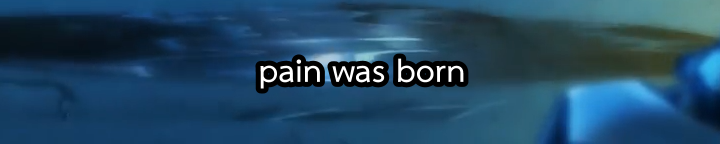
\includegraphics[width=0.8\linewidth]{images/skipborrow/currentframe.png}
			\caption{เฟรมปัจจุบัน}
			\label{image:ssim_location_curr}
		\end{subfigure}
		\bigskip
		\begin{subfigure}{0.4\linewidth}
			\centering
			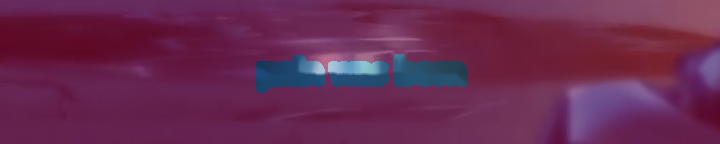
\includegraphics[width=0.8\linewidth]{images/skipborrow/prevframeinverse.png}
			\caption{บริเวณคำนวณ SSIM ของเฟรมก่อนหน้า}
			\label{image:ssim_location_prev_inv}
		\end{subfigure}
		\begin{subfigure}{0.4\linewidth}
			\centering
			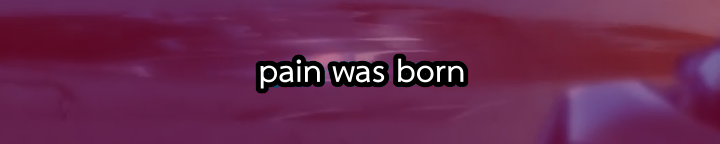
\includegraphics[width=0.8\linewidth]{images/skipborrow/currentframeinverse.png}
			\caption{บริเวณคำนวณ SSIM ของเฟรมปัจจุบัน}
			\label{image:ssim_location_curr_inv}
		\end{subfigure}
		\caption{บริเวณที่คำนวณ SSIM สำหรับการยืมเฟรมและข้ามเฟรม}
		\label{image:ssim_location}
	\end{figure}
	\hspace{1cm} จากภาพ \ref{image:ssim_location_prev} เป็นเฟรมก่อนหน้าซึ่งได้ถูกการต่อเติมภาพไปแล้ว และภาพ \ref{image:ssim_location_curr} คือเฟรมปัจจุบันที่กำลังจะต่อเติม โดยจะทำการพิจารณาค่า SSIM ในระหว่าง 2 พื้นที่แสดงในภาพ \ref{image:ssim_location_prev_inv} และ \ref{image:ssim_location_curr_inv} โดยสำหรับการข้ามเฟรม หากค่า SSIM มากกว่า 0.95 จะทำการคัดลอกภาพที่อยู่นอกพื้นที่สีแดงของภาพ \ref{image:ssim_location_prev_inv} มาแทนส่วนที่อยู่นอกสีแดงของภาพ \ref{image:ssim_location_curr_inv}  แล้วทำการข้ามเฟรมนั้นไป และสำหรับวิธียืมเฟรม หากค่า SSIM มากกว่า 0.95 จะทำการคัดลอกภาพที่อยู่นอกพื้นที่สีแดงของภาพ \ref{image:ssim_location_prev_inv} มาแทนที่โดเมนต่อเติมของเฟรมปัจจุบันแล้วจึงเริ่มการต่อเติมภาพ
	
	\hspace{1cm}ทั้งนี้ทางผู้วิจัยยังได้ทดสอบทั้ง 2 วิธีรวมกันด้วย ซึ่งจะเรียกว่าวิธีข้ามและยืม โดยเมื่อ เมื่อบริเวณนอกโดเมนต่อเติมของเฟรมปัจจุบันกับเฟรมก่อนหน้า มีค่า SSIM มากกว่า 0.95 จะให้ทำการข้ามเฟรม แต่ถ้าน้อยกว่า 0.95 แต่ยังมากกว่า 0.9 จะทำวิธีการยืมเฟรมแทน ซึ่งผลลัพธ์เฉลี่ยได้ดังตาราง
	
	\begin{table}[H]
		\centering
		\begin{tabular}[ht]{|l|c|c|c|c|}
			\hline
			วิธีการ  & เวลาประมวล  (วินาที) & PSNR (dB) & SSIM \\
			\hline
			ไม่ใช้ & 141.2850811 & 31.6037548 & 0.952397 \\
			ยืมเฟรม & 132.7787761 & 32.6481538 & 0.9658446 \\
			ข้ามเฟรม & 89.29141836 & 29.2396524 & 0.942108 \\
			ยืมเฟรมและข้ามเฟรม & 75.75894242 & 29.4711168 & 0.947267 \\
			\hline
		\end{tabular}
		\caption{แสดงผลลัพธ์เฉลี่ยของการยืมเฟรมและข้ามเฟรม}
	\end{table}	
	
	\hspace{1cm}  จากนั้นทำการทดสอบการต่อเติมวิดีโอทั้ง 5 โดยวิธีที่คิดค้นขึ้นใช้วิธีการสปริทเบรกแมนพร้อมทั้งการใช้พีระมิดรูปภาพที่มีการทำซ้ำแต่ละชั้นเป็น 10/3/3/10  พร้อมทั้งใช้การข้ามเฟรมและยืมเฟรม ได้ผลลัพธ์ออกเป็นดังตารางนี้
	 
\begin{table}[H]
	\centering
	\begin{tabular}[ht]{|l|c|c|c|c|}
		\hline
		วิธีการ  & เวลาประมวล  (วินาที) & PSNR (dB) & SSIM \\
		\hline
		สปริทเบรกแมน & * & * & * \\
		ที่คิดค้นขึ้น & 75.75894242 & 29.4711168 & 0.947267 \\
		OpenCV - Fast Marching Method & 48.64641114 & 33.0566406 & 0.9621476 \\
		\hline
	\end{tabular}
	\caption{แสดงผลลัพธ์เฉลี่ยของการลบบทบรรยายจากอนิเมะ}
\end{table}	

\hspace{1cm} สำหรับวิธีสปริทเบรกแมน เนื่องจากใช้เวลา 1 ชั่วโมงแล้วยังประมวลผลวิดีโอชุดทดสอบแรกไม่เสร็จ ทางผู้พัฒนาจึงตัดสินใจยุติการทดลอง เนื่องจากอาจต้องใช้เวลาการประมวลผลเป็นเวลาหลายชั่วโมงสำหรับวิดีโอความยาว 1 นาที ส่วนวิธีที่คิดค้นขึ้น พบว่าเวลาที่ใช้ทำงานช้ากว่าวิธี Fast Marching Method และในด้านคุณภาพ ทั้ง PSNR และ SSIM มีค่าน้อยกว่า แต่ทั้งนี้การปรับค่าพารามิเตอร์เร็กกิวลาไรต์เซซันอยู่นอกเนื้อขอบเขตการศึกษา ซึ่งหาทำการปรับพารามิเตอร์ดังกล่าวแล้ว อาจะทำให้คุณภาพที่ได้ ดีกว่าวิธีการ Fast Marching Method ได้

	
	
\section{แผนการดำเนินงานวิจัย}
\hspace{1cm} แผนการดำเนินงานตลอดทั้งโครงการสามารถสรุปได้โดยย่อจากตารางต่อไปนี้
\begin{center}
	\scalebox{0.7}{\begin{tabular}[ht]{|l|c|c|c|c|c|c|c|c|c|c|c|c|}
			\hline
			&\multicolumn{12}{c|}{เดือนที่}\\
			\cline{2-13}
			แผนการดำเนินงาน&1&2&3&4&5&6&7&8&9&10&11&12\\
			\hline
			ศึกษาตัวแบบและขั้นตอนวิธีการต่อเติมภาพที่ใช้การแปรผันรวมในเชิงลึก&x&x& & & & & & & & & &\\
			พัฒนาขั้นตอนวิธีสำหรับการต่อเติมภาพที่ใช้การแปรผันรวมชนิดใหม่& & &x&x&x&x& & & & & &\\
			ทดสอบขั้นตอนวิธีการต่อเติมภาพที่พัฒนาขึ้นโดยโปรแกรม- & & & &x &x&x& & & & & &\\
			คอมพิวเตอร์บนภาพสังเคราะห์และภาพจริง & & & & & & & & & & & &\\
			อภิปรายผลที่ได้จากการทดลองเชิงตัวเลข & & & & & &x&x&x& & & &\\
			สรุปผลการดำเนินงานวิจัยและจัดทำรูปเล่มฉบับสมบูรณ์& & & & & & & & &x&x&x&x\\
			\hline
	\end{tabular}}
\end{center}




\section{บรรณานุกรม}

\renewcommand{\section}[2]{} % addition mod: remove reference text
\begin{thebibliography}{}
	
	\bibitem{ref:rof-inpaint-chan-shen} 
	T.F. Chan and J. Shen , “Mathematical models of local non-texture inpaintings”, SIAM Journal on Applied Mathematics, vol. 62, no. 3, pp. 1019–1043, 2001. 
	%\url{http://www.jstor.org/stable/3061798}
	
	\bibitem{ref:ROF-template} 
	L. I. Rudin, S. Osher, E. Fatemi, “Nonlinear total variation based noise removal algorithms", Physica D: Nonlinear Phenomena, vol 60, issues 1–4, pp. 259-268, 1992. 
	%\url{https://doi.org/10.1016/0167-2789(92)90242-F}
	
	\bibitem{ref:FixpointSolver}
	C.R. Vogel and M.E. Oman,“Iterative methods for total variation denoising", SIAM Journal on Scientific Computing. vol. 17, pp. 227-238, 1996.
	
	\bibitem{ref:splitbergman-inpaint}
	T. Goldstein and S. Osher,“The Split Bregman Method for L1-Regularized Problems", SIAM Journal on Imaging Sciences. vol. 2, issue 2, pp. 323-343, 2009.
	
	\bibitem{ref:image-pyramid}
	E.H. Andelson and C.H. Anderson and J.R. Bergen and P.J. Burt and J.M. Ogden. "Pyramid methods in image processing". 1984
	% วิกิ บอกว่าให้ ref ของคุณ Andelson
	% doi 10.1.1.56.8646
	%\url{https://en.wikipedia.org/wiki/Pyramid_(image_processing)#cite_ref-1}
	%\url{https://en.wikipedia.org/wiki/Multiresolution_analysis}
	
	
\end{thebibliography}
\end{document}
	
	
	
	